% !TeX root = ../thuthesis-example.tex

\chapter{背景知识}

\section{社群发现}\label{sec:community_detection}

社群发现(community detection)虽然没有严格的数学定义,但公认的做法是
将现实世界的社群建模成图(graph)结构,在图结构上进行社群发现。社群根据其属性
是否随时间变化可分为静态社群和动态社群,本文研究的是静态社群,它可以用
静态图来建模,以下简称图。
一个图结构$G$ 由节点集 $V$ 和边的集合 $E$ 组成,可记为 $G(V,E)$。
根据边是否有方向可将图分为有向图和无向图。无向图可以看成是每条边
有两个方向,从而针对有向图设计的社群发现算法也可以用到无向图上面来。
此外,根据边是否有权值可将图分为有权图和无权图。有权图中节点 $i$
和节点 $j$ 之间的权值可以用 $w_{ij}$ 表示。若有权图有方向,
则 $w_{ij}$ 可以不等于 $w_{ji}$。
无向图可以看成是每条边
的权值是1,从而针对有权图设计的社群发现算法也可以用到无权图上面来。

社群发现算法根据发现的社群是否重叠可分为两类,本文研究的是非重叠的
社群发现算法,即$V$可以分为互不重叠的若干子集。

不同的社群发现算法根据自己的标准寻找社群结构,这给一般意义上的比较造成了困难。
在本节中我们介绍的社群发现算法采用的标准叫做最小化平均误差。
这个概念最早是日本学者永野清仁于2010年提出\cite{mac},但其数学形式
\footnote{与图强度的定义一致 \cite{cunningham1985optimal}}。
在这里我们采用其最为广泛的形式,即针对带权的有向图的社群发现算法。
\begin{equation}\label{eq:IP}
  \lambda_1 := \min_{\P \in \Pi'}\frac{ f[\P] }{  \abs{\P} - 1 } 
\end{equation}
在式 \eqref{eq:IP} 中,
$\P$ 表示 $V$的一个分割, 也即  $P=\{C_1, \dots, C_k\}, \cup_{i=1}^k C_i=V$。
$\abs{\mathcal{P}}$ 表示集合 $\P$ 中元素的个数。
$\Pi$ 是 $V$ 上所有分割的集合而 $\Pi'=\Pi\backslash\{V\}$ 表示 $\Pi$
除去 $V$本身.
作用在$V$的子集$C$上的函数$f$
表示$C$和 $C$的补集 $V\backslash C$ 之间边的权值之和,即
$f(C)=\sum_{i \not\in C, j\in C, (i,j) \in E} w_{ij}$。
而作用在$V$的分割$\P$上的函数 $f[\P]$ 则是$f$分别作用$\P$中每一个元素之和。
即 $f[\P]=\sum_{C \in \P} f(C)$。有了如上的符号解释,
式 \eqref{eq:IP} 即不难理解,它表示各分割之间所有边的和对分割总数的平均值。

式 \eqref{eq:IP} 实际给出了一个社群发现的标准,对于扁平化的社群而言,
最小值$\lambda_1$ 对应的社群为
分割$\P^*$的子集。

下面介绍如何求解 $\lambda_1$ 及其对应的分割$\P^*$。永野清仁 \cite{mac} 的研究指出,
求解 \eqref{eq:IP} 等价于求解下面的组合优化问题
\begin{align}\label{eq:hlambda}
  h(\lambda) &= \min_{\P \in \Pi'} f[\P] - \abs{\P} \lambda 
  \end{align}
其中 $\lambda$ 是一个非负实数。
式 \eqref{eq:hlambda} 解的结构可以由一系列嵌套的分割
来描述,即存在正整数$k$,使得式 \eqref{eq:hlambda} 的解
为:
\begin{equation}\label{eq:PSP_structure}
  h(\lambda) = \begin{cases} h_{\P_0}(\lambda) & 0\leq \lambda < \lambda_1 \\
  h_{\P_i}(\lambda) & \lambda_i \leq \lambda < \lambda_{i+1} \textrm{ for } i = 1, \dots, k-1 \\
  h_{\P_k}(\lambda) & \lambda \geq \lambda_k
  \end{cases}
\end{equation}
在式 \eqref{eq:PSP_structure} 中,$\lambda_1, \dots, \lambda_{k-1},
\lambda_k$ 是递增的数列,而 $h_{\P}(\lambda)=f[\P]-|\P|\lambda$。
对于分割 $\P_0, \dots, \P_k$ 来说,
它们也有一个序关系。我们称分割 $P$ 是 $Q$ 的一个细分,
如果 $\forall C \in P, \exists C' \in Q, s.t. C\subset C'$,
并记为 $P \preceq Q$。基于细分的此种定义,我们有:
$\P_k \preceq \dots \preceq \P_1 \preceq \P_0$。
其中 $\P_0=\{V\}$ 而 $\P_k=\cup_{i=1}^n \{ i\}$。

在得到 $h(\lambda)$ 的表达式后,
我们指出 式 \eqref{eq:IP} 和
\eqref{eq:PSP_structure} 中的$\lambda_1$ 取值
相同,因此我们用了相同的符号。而 $\P^*=\P_1$。
从而式 \eqref{eq:IP}的解可以从式 \eqref{eq:PSP_structure}
的解中获得。

下面举一个简单的例子来解释上面的结论。
\begin{example}\label{ex:psp}
考虑一个带权的有向图$G(V,E)$,其结构
如图 \ref{fig:example_directed} 所示。
试求解该图的主分割序列。
\end{example}
\begin{figure}
  \centering
  \begin{subfigure}[b]{0.5\linewidth}
  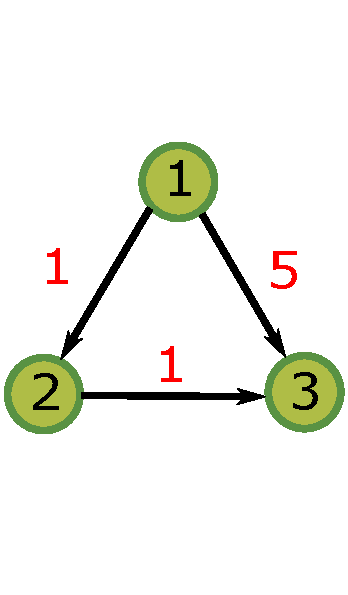
\includegraphics[width=\textwidth]{example_directed.pdf}
  \caption{一个有三个节点的带权有向图}
  \label{fig:example_directed}
  \end{subfigure}~
  \begin{subfigure}[b]{0.5\linewidth}
    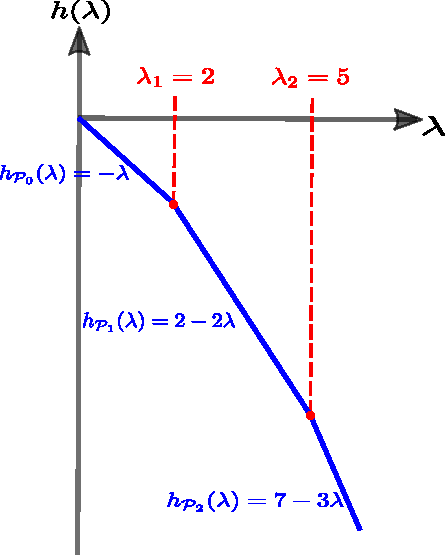
\includegraphics[width=\textwidth]{dt.pdf}
    \caption{$h(\lambda)$ 的图像}
    \label{fig:dt}
    \end{subfigure}  
\end{figure}

因为
$G$ 包含的节点只有3个,可以使用枚举法计算对应的 $h(\lambda)$
函数,其函数图像如图 \ref{fig:dt} 所示。其中
$\P_0=\{ \{1,2,3\} \}, \P_1 = \{\{1,3\}, \{2\} \},
\P_2 =\{\{1\},\{2\},\{3\} \}$。
从图\ref{fig:dt} 中可以看到,在这个简单的例子中
$h(\lambda)$
是一个分段线性函数,对于一般的图$G$对应的
$h(\lambda)$ 也是如此。

因此,基于最小平均分割的方法,\ref{fig:example_directed}
中的图将被 划分成 $\P^*=\P_1$,即节点1和3被分成一类,
而节点2单独分成1类,这符合我们的直觉。

对于一般的图,其节点数目可能很多,此时用枚举法计算
$h(\lambda)$ 变得不可行。幸运的是,计算
$h(\lambda)$ 有多项式时间的算法。下面对\cite{mac}中描述的
方法进行介绍。我们把这一方法称为 PSP 算法
\footnote{该方法最早由
印度学者 纳拉亚南 在 1991 年提出 \cite{narayanan}
},
其中
PSP 是 principal sequence of partition 的缩写,译为
主分割序列。
    
求解 \eqref{eq:PSP_structure} 只需得到在每一个
分界点处对应的 $\lambda$ 和 分割$\P$ 即可。
考虑到 $\P_k \preceq \dots \preceq \P_1 \preceq \P_0$
,
我们有 $|\P_0| \leq |\P_1| \dots \leq |\P_k|$,
即随着 $\lambda $ 的增大,线性函数的斜率逐渐增大。
这从图 \ref{fig:dt} 中也可以得到印证。
利用这一特点,我们基于分治的思想采用算法\ref{alg:psp}
获得分割序列。

\renewcommand{\algorithmicrequire}{\textbf{输入:}\unskip}
\renewcommand{\algorithmicensure}{\textbf{输出:}\unskip}

\begin{algorithm}
  \caption{求解主分割序列的算法 (PSP算法)}
  \label{alg:psp}
  \small
  \begin{algorithmic}[1]
    \REQUIRE 图$G$
    \ENSURE 序列 $L=[\lambda_1, \dots, \lambda_k]$
    和 $\mathcal{Q}=[\P_0, \dots, \P_k]$.
    \STATE \textbf{L}  $\leftarrow []$.
    \STATE $Q\leftarrow \{V\}, P \leftarrow \{ \{i \} | i \in V\}$
    \STATE $\mathbf{PSP}= [Q, P]$
    \STATE \texttt{Split}$(Q,P)$
    \STATE 对 $L$ 和 $\mathcal{Q}$
    按从小到大排序 \footnotemark
    \FUNCTION{\texttt{Split}$(Q,P)$}
     \STATE\label{alg:lambda} $\lambda' =
     {1 \over \abs{P} - \abs{Q}} (f(P)-f(Q))$
     \STATE\label{alg:lambda_plus} $h' = {1 \over \abs{P} - \abs{Q}}(\abs{P} f(Q) - \abs{Q} f(P))$
     \STATE\label{alg:lambda_f} $(\tilde{h}, P') = \texttt{DT}(G,\lambda')$
     \IF{$\tilde{h} = h'$}
       \STATE\label{algorithme:terminer} insert $\lambda'$ to $\mathbf{L}$
     \ELSE
       \STATE insert $P'$ to $\mathcal{Q}$
       \STATE\label{algorithme:gauche} \texttt{Split}$(Q, P')$
       \STATE\label{algorithme:droit} \texttt{Split}$(P',P)$
     \ENDIF
    \ENDFUNCTION
  \end{algorithmic}
\end{algorithm}
\footnotetext{$\mathcal{Q}$
中按集合的大小排序}

在算法\ref{alg:psp}第\ref{alg:lambda_f}行,
函数 \texttt{DT} 是用来求解 式\ref{eq:hlambda} 获得最优值
$\tilde{h}$ 和最优值对应的分割 $P'$。

在算法 \ref{alg:lambda}、\ref{alg:lambda_plus} 行,
求解 $(\lambda', h')$ 相当于在二维 $(\lambda, h)$
平面上计算直线
$h = f[P] - |P| \lambda $
和 $h = f[Q] - |Q| \lambda $ 的交点。假设 $P, Q$ 对应的
分界点分别是 $\lambda_P, \lambda_Q$(约定 $\{V\}$ 对应 0,
$\{\{i\}|i\in V\}$ 对应 $+\infty$),那么根据几何直观
$\lambda_Q \leq \lambda' \leq \lambda_P$。
紧接着,\ref{algorithme:gauche} 行的调用对应在
$[\lambda_Q, \lambda']$
区间范围内寻找剩余的分界点,而
\ref{algorithme:droit} 行的调用对应在
$[\lambda', \lambda_P]$
区间范围内寻找剩余的分界点。最后,
\ref{algorithme:terminer} 行表明
$[\lambda_Q, \lambda_P]$ 内没有分界点,无需再调用
\texttt{Split} 函数。

如前所述,函数 \texttt{DT}
(Dilworth truncation,迪尔沃思截断\footnote{采用迪尔沃思截断
这个名称是沿用了文献\cite{mac}中的称谓})
是用于求解式\eqref{eq:hlambda}的算法,它实际上是一种贪心算法,
由算法\ref{alg:dt} 给出。

\begin{algorithm}
  \caption{迪尔沃思截断算法}\label{alg:dt}
  \begin{algorithmic}[1]
  \REQUIRE 图 $G$ 和 $\lambda$
  \ENSURE 分割 $\P$ 和 $h$
  \STATE
  $V^0 = \emptyset, x $ 是 $n$ 长的向量\footnotemark,
  $\mathcal{A} = \{\}$
  \FOR{$l=1, 2, \dots, n$}
  \STATE $V^l = \{l\} \cup V^{l-1}$
  \STATE\label{alg:tight} 计算 $x^* = \displaystyle\min_{ A: l \in A \subseteq V^l} f(A)- x(A)$。
   $T^l$ 是达到此最小值的集合,并且 $x_l \leftarrow x^* - \lambda$。 
    \STATE $U^l = T^l \cup [\cup \{A | A \in \mathcal{A}, A \cap T^l \neq \emptyset\}] $
  \STATE $\mathcal{A} = \{U^l\} \cup \{A | A \in \mathcal{A}, A \cap T^l = \emptyset \}$
  \ENDFOR
  \STATE $\P^* = \mathcal{A}, h_{\lambda} = x(V)$
  \end{algorithmic}
  \end{algorithm}
\footnotetext{$n$ 是图$G$中节点的个数}

算法\ref{alg:dt}涉及到一种新的运算记号$x(A)$,
这里 $x$ 表示一个向量而 $A$ 是一个集合
$x(A)$ 定义为 $\sum_{i \in A} x_i$。
此外,采用\cite{pin}中的方法,我们可以把\ref{alg:tight} 行中的最优化
问题转化成有向图上的最大流问题。
具体而言,
针对 $\displaystyle\min_{ A: l \in A \subseteq V^l} f(A)- x(A)$,
我们首先构造一个图$G'$包含节点$V'=\{0, 1, 2, \dots, l\}=\{0\} \cup V^l$。
节点 $0$ 是相对新加入的,作为最大流算法的源节点。
而$l$是目标节点。图$G'$中有向边的权值有如下定义:
\begin{equation}\label{eq:wij_prime}
  w'_{ij} = \begin{cases}
    \max\{0, -x_{i}\} & \textrm{ if } i = 0 \\
    \max\{0, -x_{i}\} + w_{il} & \textrm{ else if } j = l \\
    w_{ij} & \textrm{ otherwise }
  \end{cases}
\end{equation}

按照定义式 \eqref{eq:wij_prime}, 源节点0和目标节点j
之间的权值为零,即两节点间没有边相连。
基于定义好的图$G'$和$s=0,t=l$,我们求解如下
标准的最小割问题:
\begin{equation}\label{eq:mincut}
  \beta = \min_{A \subseteq V^l: l\in A }
  c(V' \backslash A, A)
\end{equation}

达到式\eqref{eq:mincut}
最小值的集合即是 $T^l$,并且$x^*$和 $\beta$
有如下关系式:
\begin{equation}\label{eq:beta_alpha}
  \beta = x^* + \sum_{x_v > 0, 1\leq v < l} x_v
\end{equation}

\section{信息聚类}
在信息论领域,互信息提供了两个随机变量之间的
距离度量。使用 KL 散度的记号,随机变量$X$
和 $Y$ 之间的互信息定义为:
\begin{equation}\label{eq:mutual_info}
  I(X;Y) = D(P_{XY} ||P_XP_Y)
\end{equation}
其中 $P_X, P_Y$分别表示边缘分布,而$P_{XY}$
表示两个随机变量的联合分布。有多种方法可将互信息
的概念推广到两个及以上的随机变量,
其中华人学者陈聪提出了一种推广 \cite{ska} 具有多种好的性质,
且涵盖了图结构的情形,我们把他的推广叫做多变量互信息,英文全称是
Multivariate Mutual Information (MMI)。

下面我们对MMI做简要的介绍。定义$V$是随机变量
的序号集合,$C$是 $V$的子集,$Z_C=\{Z_i | i \in C\}$
表示随机变量序号在 $C$ 中的随机变量 $Z_i$ 的集合。
$\P$ 表示$V$ 的一个分割,$P_{Z_C}$表示$Z_C$
的联合分布。$\Pi'(V)$ 是
除去$\{V\}$外所有$V$的分割的集合。MMI的度量定义为:
\begin{align}
  I(Z_V) &:= \min_{\P \in \Pi'(V)} I_{\P}(Z_V) \textrm{ where } \label{eq:IZV}\\  
  I_{\P}(Z_V) &:= \frac{1}{|\P| - 1}D(P_{Z_V} || \prod_{C\in \P} P_{Z_C}) \label{eq:IPZV}
\end{align}
在上面的定义中,如果$Z_V$彼此独立,那么$I(Z_V)=0$,
反之亦然。

式\eqref{eq:IPZV}给出了特定分割下的多变量互信息,
也可根据下式把KL散度改写成熵的形式。
\begin{equation}\label{eq:entropy_expression}
  D(P_{Z_V} || \prod_{C\in \P} P_{Z_C}) 
  = \sum_{C \in \P}
  H(Z_C) - H(Z_V)
\end{equation}
对于一般的分布,式\ref{eq:IZV}
难于计算。陈聪提出了一种特殊的PIN模型\cite{pin}\footnote{PIN 是 pairewise independent network
的缩写},
使得多变量互信息可以用\ref{sec:community_detection}节
介绍的PSP算法进行计算。
这里略去PIN模型的数学定义,而是通过下面的例子
阐发它和图结构的联系。
\begin{example}\label{ex:mmi}
  令$V=\{1,2,3\}$,$Z_1=(X_a, X_c)$,
  $Z_2=(X_a,X_b)$ 且 $Z_3=(X_b,X_c)$。
  $X_a,X_b,X_c$是独立的随机变量且它们的熵分别为:
  $H(X_a)=H(X_b)=1, H(X_c)=5$。
  利用联合熵的公式不难计算出$H(Z_1)=H(X_a)+H(X_c)$以及
  $H(Z_1, Z_2) = H(X_a) + H(X_b) + H(X_c)$等。
  若 $\P=\{\{1,2\}, \{3\}\}$,则根据
  \eqref{eq:entropy_expression}式,
  $D(P_{Z_V}||P_{Z_1,Z_2}P_{Z_3}) = H(X_a)
  +H(X_b)$。我们可以将上面的计算用图\ref{fig:example_directed}
  进行对应,即把$Z_i$对应到第$i$的节点,
  $Z_i$与$Z_j$之间的互信息对应到第$i$和第$j$个节点之间
  边的权值,而KL散度即为不同的类别之间边的权值之和。
\end{example}
例\ref{ex:mmi}中虽然只有三个节点,
但对于一般的情形,PIN模型也是和一个有向图有
着类似的对应关系。因此,在PIN模型下多变量互信息可以用
PSP算法进行计算。

基于MMI可以对随机变量进行聚类,聚类簇
定义为
\begin{align}
  C(Z_V) &:= \bigcup_{\gamma \in \R} C_{\gamma}(Z_V)
  \label{eq:czv}\\
  C_{\gamma}(Z_V) &:= \textrm{maximal}
  \{ B \subseteq V \big\vert |B|>1, I(Z_B) > \gamma  \}
\end{align}
理论分析表明,基于定义式\ref{eq:czv} 可以得到和
式\ref{eq:PSP_structure}类似的层次聚类结果。
即存在一系列的临界值$\lambda_1 < \dots < \lambda_k$和分割
$\P_k \preceq \dots \preceq \P_0$,使得
$C(Z_V) = \bigcup_{i=1}^{k} C_{\lambda_i}(Z_V)$
且$C_{\lambda_i}(Z_V) = \P_i$。

有两种生成聚类簇的方法,它们均可以通过聚类树
来描述。聚类树可看成是一系列
嵌套的分割$\P_i$的另一种描述方式。
聚类树有一个根节点$V$,
其所有的叶节点为 $\{j\}$,其他节点均对应着
一个聚类簇。

\begin{description}
  \item[自顶向下] 假设 $I_{\P^*}(Z_V)=I(Z_V)$, 
  把 $\P^*$ 中每一个元素作为 $V$ 的子节点。
  对于每一个子节点$C$,求解$I(Z_C)=I_{\P_C}(Z_C)$
  并使用分割 $\P_C$ 对子树进一步细分直到子节点变成单元素集为止。
  \item[自底向上\footnotemark] 假设 $I(Z_C) = \max_{B\subseteq V} I(Z_B)$ 并且 
  将 $C$ 中所有的元素合并成一个作为聚类树的子节点。对于当前所有子节点,找到MMI
  最大的集合进行合并直到所有子节点合并成根节点$V$为止。
  \end{description}
  \footnotetext{参见\cite{agg_ic}}

  \begin{figure}[!ht]
    \centering
    \begin{subfigure}[b]{0.38\linewidth}
      \centering
      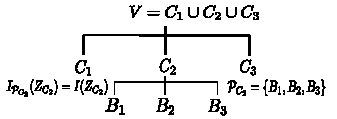
\includegraphics[width=\textwidth]{top_down.pdf}
      \caption{}\label{fig:top_down}
    \end{subfigure}~
  \begin{subfigure}[b]{0.33\linewidth}
    \centering
    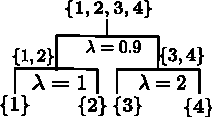
\includegraphics[width=\textwidth]{threshold_a.pdf}
    \caption{}\label{fig:threshold_a}
  \end{subfigure}~
  \begin{subfigure}[b]{0.29\linewidth}
    \centering
    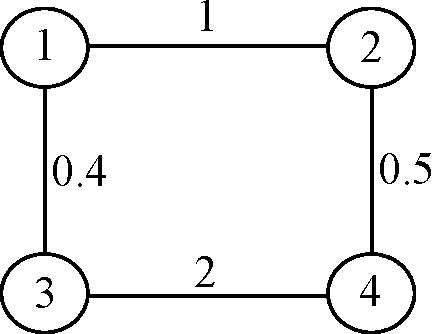
\includegraphics[width=\textwidth]{threshold_b.pdf}
    \caption{}\label{fig:threshold_b}
  \end{subfigure}
    \caption{聚类树示例}\label{fig:mmi_example}
  \end{figure}
自顶向下
获得聚类树的示意图由图 \ref{fig:top_down} 给出。
下面我们用一个简单的例子来说明聚类树的结构。
  \begin{example}\label{ex:mmi_tree}
考虑图\ref{fig:threshold_b}所示的情形,
$V=\{1,2,3,4\}$。互信息在图的边上标出,
比如 $I(Z_1;Z_2)=1, I(Z_1;Z_4)=0$。
利用定义式\ref{eq:IZV}不难求出
$I(Z_V)=0.9$。 
我们可以写出完整的聚类结果:
\begin{equation*}
\P = 
\begin{cases}
\{\{1,2,3,4\}\} & \lambda < 0.9 \\
\{\{1,2\},\{3,4\}\} & 0.9 \leq \lambda < 1 \\
\{\{1\},\{2\},\{3,4\}\} & 1 \leq \lambda < 2\\
\{\{1\},\{2\},\{3\},\{4\}\} & \lambda \geq 2
\end{cases}
\end{equation*}
把各临界值$\lambda_i$ 标到聚类树上即如图
\ref{fig:threshold_a}所示。
\end{example}

\section{参数化的最大流算法}
最大流算法用于解决网络流中从一点到另一点的最优运输路径的问题。
其中一类基于前置推送-标签重贴(push-relabel) \cite{Goldberg1988} 的算法
具有良好的效率。如果要解一系列的最大流问题并且这一系列的问题
之间有一定的关联性,重复调用最大流算法显然不是最优的选择。
基于这种考虑,有学者提出了参数化的最大流算法\cite{Gallo1989}用于求解
具有特殊结构的一系列的最大流问题。下面对参数化的最大流算法
进行简单的介绍。

首先让我们回顾一下最大流问题。
考虑一有向图$G(V,E)$。其节点集$V$
中包含两个特殊的节点:源节点$s$
和目标节点$t$。对每一对有向边
$(u,v)$存在一个非负的容量函数
$c(u,v)$。如果$u,v$之间没有有向边
定义$c(u,v)=0$。
最大流问题是求解流量函数
$f(u,v)$,使得$\sum_{v\in V} f(v,t)$
最大。流量函数需要满足如下约束
\begin{align}
  f(u, v) \leq c(u, v) \textrm{ for } (u, v) \in V \times V \\
  f(u, v) = -f(v, u) \textrm{ for } (u, v) \in V \times V \\
  \sum_{v \in V} f(u,v) = 0 \textrm{ for } v\in V\backslash\{s, t\}
\end{align}
最大流和形如式\eqref{eq:mincut}所示的最小割问题
互为对偶问题。因此求解最大流问题的算法也可以
用于求解最小割问题。

参数化的最大流算法考虑的问题是在最大流问题的
基础上,假设$c(s,v)$ 
是关于$\lambda$的增函数
且$c(v, t)$是$\lambda$的减函数,
分别记为
$c_{\lambda}(s,v)$ 和 $c_{\lambda}(v, t)$。
对于一系列的$\lambda_1 < \dots < \lambda_k$,
我们可以得到 $k$ 个最大流问题。参数化的最大流算法
即基于前置推送-标签重贴算法,通过保留
在$\lambda_{i-1}$上的计算状态并用于下一步的初始化,
以及适当地使用并行化的技术,使得计算$k$ 个最大流问题
的时间复杂度和只计算一个最大流问题近似相等。
\citet{kolmogorov} 提出一种方法,将求解式\ref{eq:hlambda}
转化为求解n次参数最大流问题。
这种方法与算法\ref{alg:dt}的思路不一样,
因为其基于参数化最大流,
我们称之为PMF算法
\footnote{PMF 是 parametric maximal flow 的缩写}。

\section{局部信息几何}
KL散度可用于度量两种不同概率分布
之间的距离。当这两种分布比较接近时,
局部信息几何刻画了KL散度的近似表达式。
下面我们以离散分布为例,给出分布之间距离的接近的
形式化定义。
$P_0$ 表示概率质量函数 (PMF),其定义域为字母集$\mathcal{X}$。
我们称 $P$ 在 $P_0$的 $\epsilon$ 邻域 $N^{(\epsilon)}(P_0)$ 内,如果
\begin{equation}
P \in N^{(\epsilon)}(P_0) \iff \sum_{x \in \mathcal{X}} \frac{(P(x) - P_0(x))^2}{P(x)} < \epsilon^2
\end{equation}
